\chapter{Registrierung mit PHP}
Die Registrierung eines Users wurde mit PHP umgesetzt, dabei wurde zuerst ein einfaches HTML-Formular erstellt, um die vom User eingegebenen Registrierungsdaten an den Server zu \"ubertragen, wobei es ebenfalls zur Auswertung des HTML-Formulars durch den Server kommt. 
Das nachfolgende Listing zeigt das HTML-Formular:
\newline
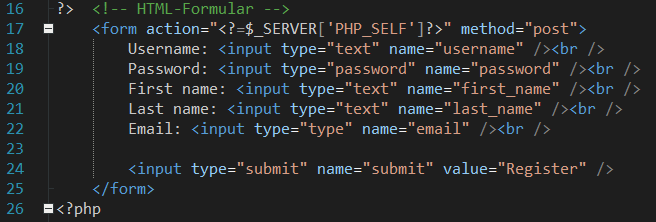
\includegraphics[width=1\textwidth]{img/vincent/abb11.png}
\newline
Wie aus dem Code zu entnehmen ist, werden f\"ur die Registrierung Username, Passwort, Vor- und Zuname und die Email-Adresse des Users \"ubertragen. Durch die Definition des Passwort Eingeabefeld mit \textit{type="password"} wird ein maskieren der eingegebenen Zeichen mit Punkten erreicht wie folgende Abbildung zeigt:
\newline
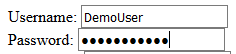
\includegraphics[width=0.5\textwidth]{img/vincent/abb01.png}
\newline
Nachdem der User seine Daten zur Registrierung eingegeben hat, werden diese an den Server gesendet. Der Server baut eine Verbindung zur \textit{MySQL}-Datenbank auf, dabei greift er auf eine zuvor erstellte Konfigurationsdatei zu und liest die ben\"otigten Informationen wie z.B. denn Datenbankuser und dessen Passwort aus. Anschlie{\ss}end wird die Verbindung zu Datenbank \"uberpr\"uft. Das nachfolgende Listing zeigt die beschriebene Funktion:
\newline
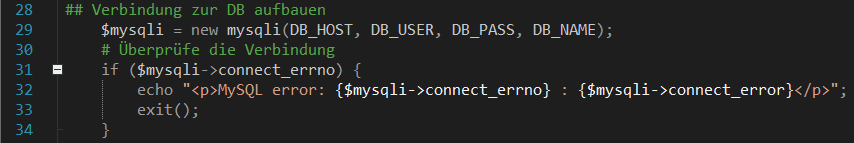
\includegraphics[width=1\textwidth]{img/vincent/abb12.png}
\newline

Nachdem die Verbindung zur Datenbank \"uberpr\"uft wurde, wird eine Datenbankabfrage vorbereitet, dabei werden die Daten des HTML-Formulars in Variablen gespeichert. Nun wird mittels einer Else-If-Verzweigung \"uberpr\"uft, ob ein User mit dem selben Usernamen oder derselben Email-Adresse bereits existiert, damit sich kein User mit denn selben Informationen ein weiteres Mal registrieren kann und die Datenkonsistenz gew\"ahrleiset ist. Durch das \textit{echo}-Kommando wird eine entsprechende Information ausgegeben, sollte es bereits existente Eintr\"age geben. Folgendes Listing zeigt den beschriebenen Code:
\newline	
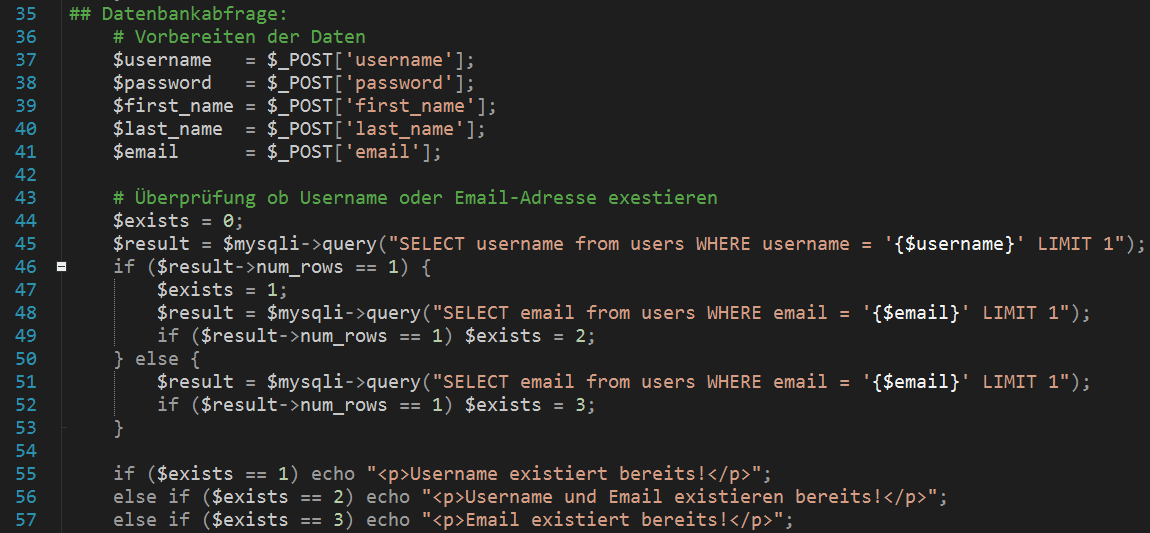
\includegraphics[width=1\textwidth]{img/vincent/abb13.png}
\newline

Nachdem sichergestellt wurde, dass die Daten f\"ur die Erstellung eines neuen Users geeignet sind, wird ein neuer Datenbankeintrag mit den Daten aus dem HTML-Formular erstellt. Anschlie{\ss}end wird eine Meldung ausgegeben, welche dem User mitteilt, das die Registrierung erfolgreich war:
\newline	
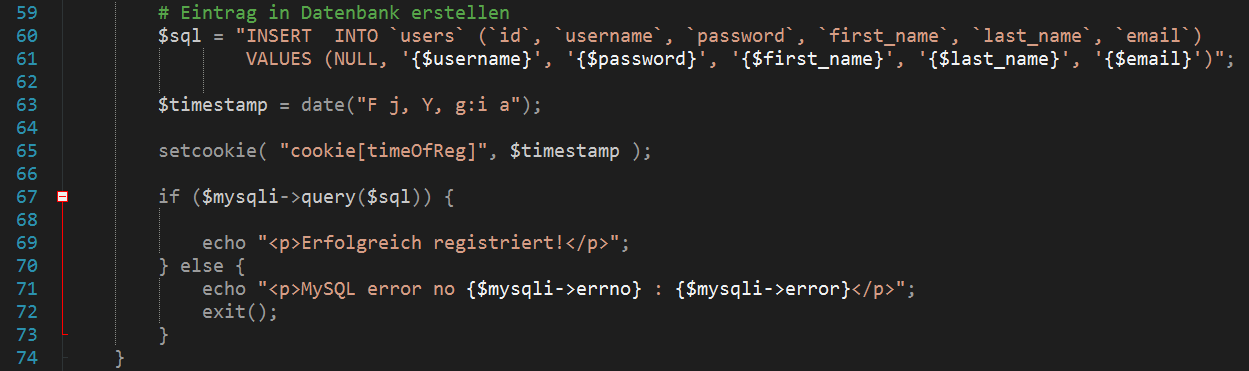
\includegraphics[width=1\textwidth]{img/vincent/abb14.png}
\newline
Im Coding wird auch ein Cookie gesetzt, dazu mehr im Abschnitt, welches sich mit dem Setzen und der Auswertung eines Cookies besch\"aftigt.	

\chapter{Websockets zur Systemzeitabfrage}
Eines der Ziele des Projekts war die Implementierung von Websockets, diese wurde mittels \textit{node.js} und der Bibliothek \textit{node.js-websocket}
auf der Serverseite und mittels Javascript auf der Clientseite umgesetzt. Der Server horcht auf eingehende Verbindungen auf dem Port 8001. Sobald sich ein Client verbunden hat wird eine Event gefeuert und der Server sendet seine Systemzeit \"uber die Websocket-Verbindung an den Client, wie aus folgendem Coding zu entnehmen ist:  
\newline
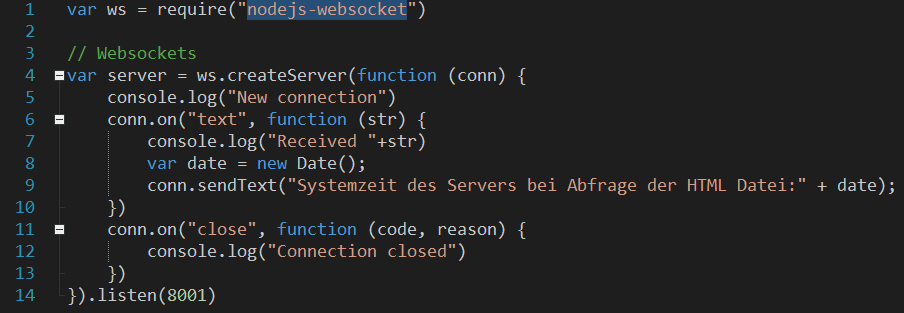
\includegraphics[width=1\textwidth]{img/vincent/abb02.png}
\newline
Auf der Clientseite wird mittels Javascript ein Websocket erstellt, welcher ebenfalls Events feuert. Sobald die Verbindung aufgebaut ist, wird eine Probenachricht an den Server gesendet. Der Server wiederum sendet seine Systemzeit, diese wird dann mittels \textit{document.getElementById} f\"ur den User im Frontend dargestellt: 
\newline
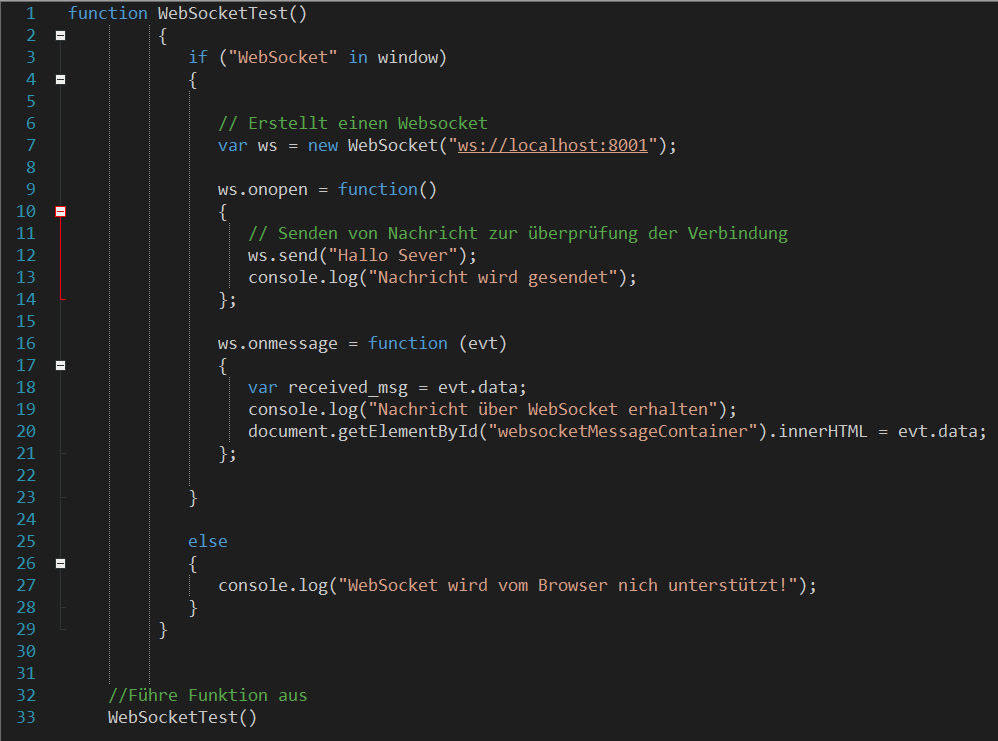
\includegraphics[width=1\textwidth]{img/vincent/abb03.png}
\newline
Das Ergebnis sieht wie folgt aus:
\newline

\includegraphics[width=1\textwidth]{img/vincent/abb17.png}
\newline
\chapter{Minispiel per Canvas}
Mittels Canvas wurde ein kleines Spiel f\"ur den Zeitvertreib implementiert. Dabei wurde zuerst ein Canvas-Element und grundlegende Funktionen definiert um z.B. den Inhalt des Canvas-Elements zu löschen, diese Funktion wird mittels \textit{setInterval} immer wieder aufgerufen, damit das Canvas neu gezeichnet werden kann.     
\newline
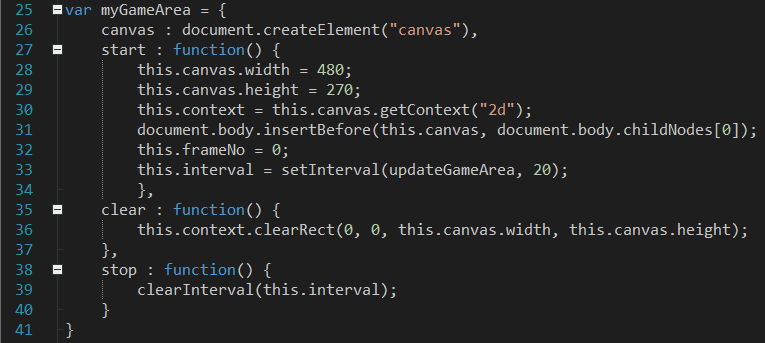
\includegraphics[width=1\textwidth]{img/vincent/abb04.png}
\newline
Durch die \textit{Component} Funktion werden die Objekte, wie z.B. der Hintergrund und der Taucher erzeugt, dabei werden Bilddateien geladen, wie im folgender Abbildung zu erkennen ist: 
\newline
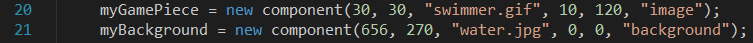
\includegraphics[width=1\textwidth]{img/vincent/abb05.png}
\newline
Die \textit{Component}-Funktion erh\"alt als Parameter die Koordinatenposition des \"ubergebenen Elements, wenn es sich um ein Bild handelt, wird mittels \textit{new Image()} ein Bild zum zeichnen auf dem Canvas erstellt. In der \textit{Update}-Funktion wird das Bild letztendlich gezeichnet, da diese Funktion mehrmals die Sekunde aufgerufen wird entsteht die Illusion einer Bewegung des Tauchers und des Hintergrundes. Dabei wird mittels der \textit{newPos}-Funktion daf\"ur sorge getragen, dass sich die logische Position des Bildes ver\"andert, die Variable \textit{speedY} und \textit{speedX} geben die Geschwindigkeit an mit der die Position ver\"andert wird. 
\newline
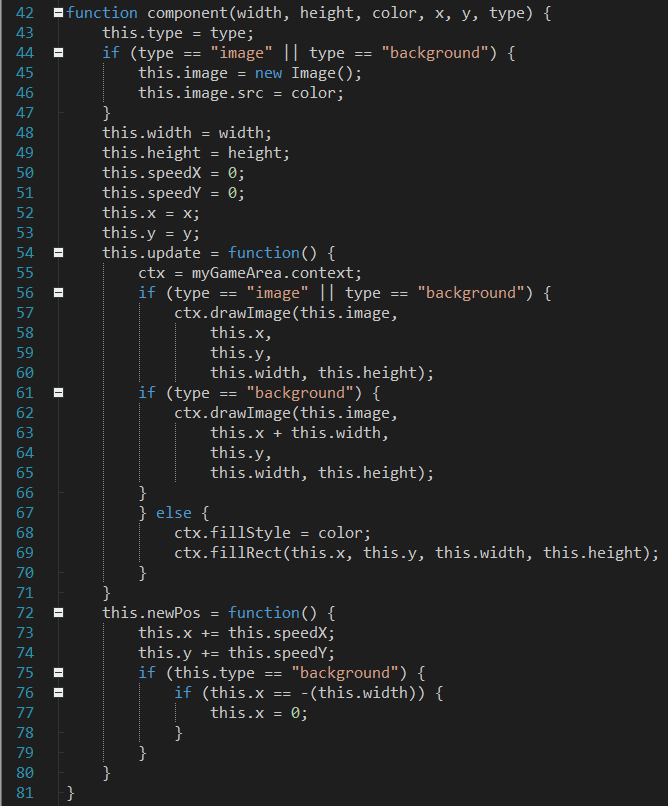
\includegraphics[width=1\textwidth]{img/vincent/abb06.png}
\newline
Den Motor des Programms bildet die \textit{updateGameArea}-Funktion. Sie wird per \textit{setInterval} alle 20 Millisekunden aufgerufen, und aktualisiert die Position des Hintergrunds und die des Tauchers, außerdem sorgt sie daf\"ur das die \textit{Update}-Funktionen ausgef\"uhrt werden:
\newline
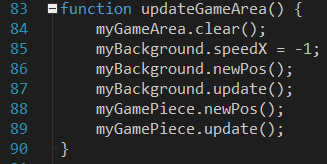
\includegraphics[width=0.6\textwidth]{img/vincent/abb07.png}
\newline
Der User kann die Bewegung des Tauchers per Buttons steuern, dabei wird die Geschwindigkeit des Tauchers, je nachdem welcher Button gedr\"uckt wurde entsprechend ver\"andert:
\newline
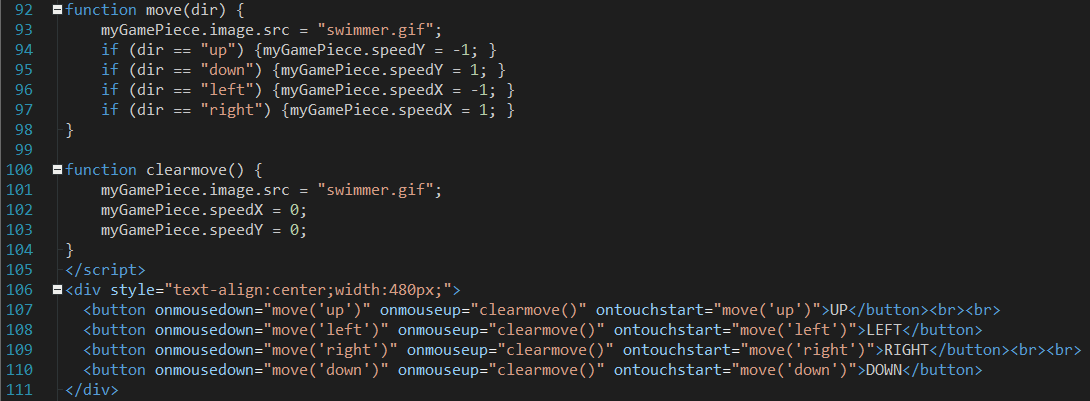
\includegraphics[width=1\textwidth]{img/vincent/abb08.png}
\newline
Das Endergebnis l\"asst sich in nachfolgender Abbildung bewundern:
\newline
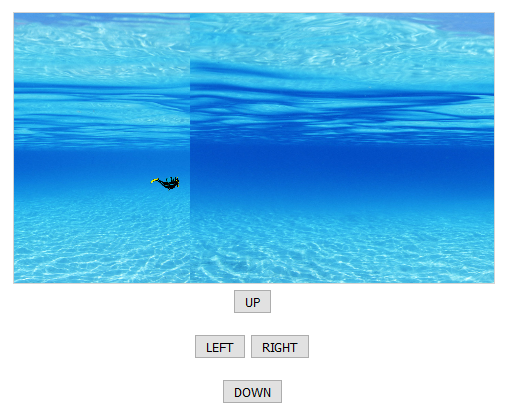
\includegraphics[width=0.7\textwidth]{img/vincent/abb09.png}
\newline
\chapter{Serverseitige Bildgenerierung}
Um die serverseitige Bildgenerierung mittels php durchzuf\"uhren, wurde eine neue php-Datei erstellt. Diese soll bei Aufruf ein Banner erzeugen, welches dann in die Hauptseite eingebunden wird. Dabei wird der Text 'Viel Erfolg bei den Wettk\"ampfen!' verwendet, welcher in zuf\"alliger Farbe angezeigt wird, es wird außerdem ein eigener Font genutzt. durch die rand Funktion wird ein zuf\"alliger Farbwert generiert und anschließend verwendet um die Textfarbe festzulegen. Am Anfang wird nnoch \"uberpr\"uft, ob bereits ein entsprechendes Bild generiert wurde, wenn dass der Fall ist, wird dieses \"uberschrieben, dadurch wird dem User bei jedem Aufruf der Seite ein Banner in anderer Farbe angezeigt. Folgendes wurde programmiert:
\newline
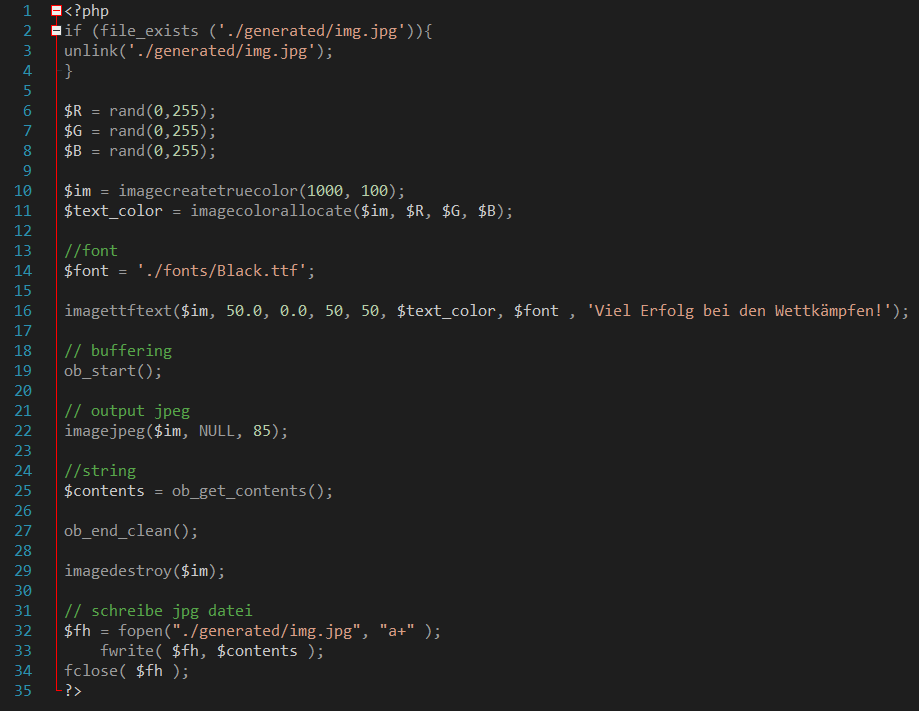
\includegraphics[width=1\textwidth]{img/vincent/abb10.png}
\newline
Hier zwei Beispiele f\"ur das Ergebnis der Generierung:
\newline

\includegraphics[width=1\textwidth]{img/vincent/img.jpg}

\includegraphics[width=1\textwidth]{img/vincent/img2.jpg}
\newline
\chapter{Cookie für den Registrierungszeitpunkt}
Ein weiteres Ziel des Projektes war die sinnvolle Verwendung eines Cookies, mittels php wurde ein Cookie bei der erfolgreichen Registrierung gesetzt:
\newline
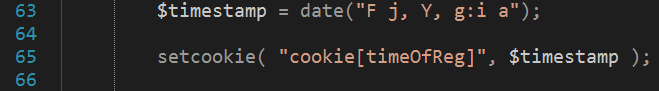
\includegraphics[width=1\textwidth]{img/vincent/abb18.png}
\newline
Wie aus dem Coding zu entnehmen ist, wurde dabei der Zeitpunkt der Registrierung im Cookie gespeichert. Das Auswerten des Cookies findet beim erneuten Aufruf der Website statt:
\newline
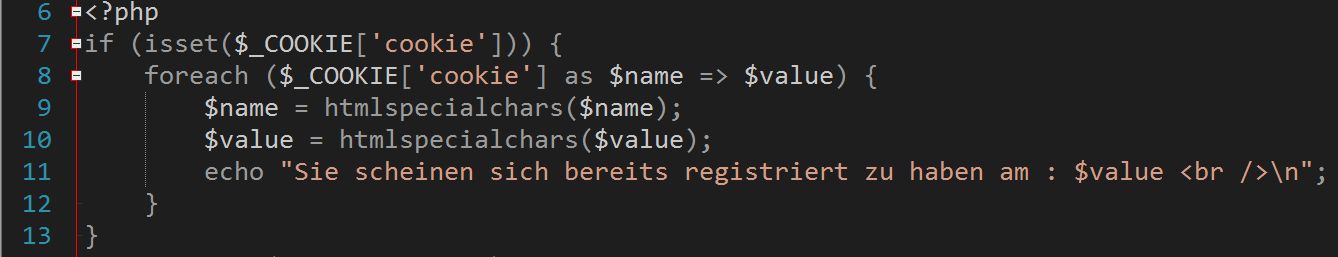
\includegraphics[width=1\textwidth]{img/vincent/abb19.png}
\newline
Dem User wird angezeigt, ob er sich mit hoher Wahrscheinlichkeit schon registriert hat, zus\"atzlich wird der Zeitpunkt der Registrierung ausgegeben. Folgendes Ergebnis wird dem User angezeigt:
\newline
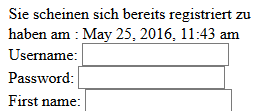
\includegraphics[width=0.6\textwidth]{img/vincent/abb20.png}
\newline

